\chapter{Real-time komunikace}
Real-time \index{Real-time} komunikace představuje významný prvek v aplikacích, kde je zapotřebí přesných časových rámování přenášeného signálu. Real-time systém je buď hardwarový nebo softwarový systém, který by měl komunikovat s řídícím systémem v přesně stanovených časových periodách. Tato definice tedy neznamená, že by měl systém odpovídat, nebo posílat data okamžitě, ale že garantuje reakci systému v daném časovém intervalu a to buď reakcí na výzvu od řídícího signálu, nebo ve fixní časy (tedy v relativní nebo absolutní čas) \cite{real-time}. Dále lze real-time komunikaci rozdělit na tzv. soft real-time a hard real-time. Rozdíl je pouze v samotném přístupu ke spolehlivosti přenosu informace. U soft real-time přístupu je možné připustit, že se informace po nějakém čase zahodí, jelikož je již nežádoucí. Jinými slovy, pokud informace nedorazí do přijímače v určitém čase, postrádá svojí informační hodnotu. Toto by měl však být pouze ojedinělý stav. U hard real-time toto není přípustné. Tento přístup se hodí pro aplikace vyžadující velmi vysokou spolehlivost a je tak méně častý.

Obecně lze však za real-time aplikaci uvažovat systém, který reaguje na požadavky bez zbytečného dopravního zpoždění, které je například u webových aplikací naprosto běžné a odezvy v přesně definovaných časových odezvách se nepoužívají zejména z důvodu rychlosti. Je totiž mnohem dů\-le\-ži\-těj\-ší odeslat data ze serveru co nejrychleji, než je posílat podle časově definovaných oken. Předejít však dopravnímu zpoždění u webových aplikací není možné. Důvod je prostý. Webová aplikace musí být dostupná pro všechny uživatele na celém světě a z toho plyne, že každý uživatel je na jiném geografickém místě a čas potřebný k dostání informace ke koncovým uživatelům není stejný. Tento problém lze částečně vyřešit distribuovaným systémem, kdy se servery přibližují uživatelům, což prakticky dělají například streamovací portály jako je YouTube. Toto řešení má svá omezení a proto druhým způsobem, jak ušetřit čas při komunikaci s koncovým prvkem, je zjednodušit komunikační protokol, nebo se omezit na co nejméně zbytečné režie a to i za tu cenu, že nedojde ke stoprocentnímu přenosu informace.

\section{Hardwarové prostředky senzorické sítě}
Požadavky na hardwarové prostředky této sítě nejsou v současné chvíli, zadávající firmou této práce, nijak definovány. Je tedy možné síť navrhnout libovolným způsobem. Vzhledem ke komplikovanosti celé problematiky bude v rámci této práce popisována síť jako striktně metalická paketová. Veškeré informace však platí bez významnějších změn i pro bezdrátová připojení. Taková síť se tedy skládá v nejmenší konfiguraci pouze z koncového členu a serveru. S narůstajícím počtem koncových členů je zapotřebí síť patřičně rozšiřovat. Výhodou tohoto systému je fakt, že se daná síť nijak neliší od běžných metalických ethernetových sítí, tzn. že lze využít veškeré dostupné prostředky pro tvorbu této sítě a není zapotřebí vyvíjet zbytečně drahá nová zařízení.

Celá síť se tak skládá z klasického ethernetového vedení a rozbočovačů, přepínačů popř. směrovačů. Zbývá tedy vyřešit server a koncové členy. Zde však záleží na praktické aplikaci. Vezmeme-li však v úvahu nejobyčejnější systém, server pak může být prakticky jakýkoliv počítač, který dokáže zpracovat příchozí požadavky. Tzn. musí být dostatečně výkonný a pro lepší bezpečnost celého systému také redundantní (nebo alespoň některé kritické komponenty v něm). Redundanci komponent však dobře řeší klasické servery, kde jsou redundantní například zdroj, pevné disky, řadiče a dále duální paměti popř. procesory.

Samotné koncové prvky se pak sestávají z nízkoodběrových mikrokontrolérů, \index{Mikrokontrolér} které mají menší, pro danou aplikaci však dostatečný výkon. Zde opět záleží na daném účelu koncového zařízení. Pokud má sloužit jako koncentrátor, tedy zařízení sbírající data ze senzorů, potřebuje větší výkon než například termální čidlo. Obecně však platí, že zařízení musí být dostatečně výkonná, aby bylo možné využívat bezdrátového připojení, nebo Ethernetu. \index{Ethernet} Potřebný výkon koncového prvku je tak dán samotným programem, který na tomto prvku poběží a dále potřebnou periferií pro připojení k serveru.

Tato síť je tedy v takovém stavu, kdy je zapojen server (nejlépe na nezávislém napájení) a senzory jsou zapojeny v ethernetové síti pomocí běž\-ných síťových prvků. Důležité je však vyřešit co se stane, když vypadne napájení? V tomto okamžiku síť prakticky přestane fungovat. Toto se nijak neliší od např. běžné zapojení elektroinstalace. Sice by šlo zajistit napájení koncových prvků, protože server může být zapojen na více nezávislých zdro\-jích elektrické energie, to však nebude např. v rodinném domě běžné. Horší případ nastane, když vypadne připojení k internetu. Zde by se nejednalo o problém, pokud by se server nacházel v řízeném objektu. Jediný efekt by byl ten, že by nebylo možné server ovládat vzdáleně. Horší situace ovšem nastane v okamžiku, kdy je server umístěn ve vzdálené serverovně. V takovém případě je pro tuto senzorickou síť potřeba vyřešit chování v případě poruchy (tzv. disaster solution). Samotné koncové členy musí vědět jak se chovat bez příchozího signálu. To většinou není problém, protože paradoxně není potřeba řešit jejich chování. To je nutné pouze v případě zabezpečení objektů. Starostí koncových členů totiž není např. vypnout světlo, pokud není systém připojen k internetu. V takovém objektu je však zapotřebí zařadit do sítě zařízení, které bude přijímat od serveru povely a obsluhovat síť. V případě přerušení spojení se serverem převezme toto zařízení kontrolu nad sítí a uvede objekt do dočasného módu, než se problém vyřeší, nebo než přijede servis. Bude tak možné i nadále ovládat alespoň na základní úrovni většinu zařízení.

\section{Real-time ve webových aplikacích}
Ve webových aplikacích žádný real-time \index{Real-time} jako takový v podstatě neexistuje. Existují však technologie, které umožňují rychlou komunikaci s webovým serverem, resp. rychlou výměnu dat, což vždy nemusí být jedno a to samé. Je totiž rozdíl mezi tím, jestli je nutné při každém požadavku sestavovat nové spojení se serverem, nebo je možné bez další režie rovnou vyměňovat data.

Jedním z typických zástupců je AJAX (popř. AJAJ). Jedná se jed\-no\-směr\-ný mechanismus, kdy se po periodické akci, nebo například při stisku tlačítka vyvolá javascriptová akce, která uzavře HTTP spojení se serverem a získá data v závislosti na požadavku. Následně překreslí část stránky obsahující nová data. Nedojde tak k obnovení celé stránky, ke kterému by došlo při běžném pohybu návštěvníka na stránce. Výhodou je, že není zapotřebí přenášet celou stránku. Nevýhodou však je možný nárůst HTTP požadavků na server a hlavně nutnost vyjednat se serverem spojení při každém po\-ža\-dav\-ku, což je časově velmi náročné. Pro tuto aplikaci je proto použití AJAXu nevhodné. \index{AJAX}

Oproti tomu websocket \cite{rfc6455} je protokol, který umožňuje otevřít socket mezi serverem a prohlížečem a pomocí rámců posílat obousměrně informace. Vyjednat spojení se serverem tak stačí pouze jednou při otevření webové stránky a následně je možné velmi rychle se stránkou komunikovat. Zároveň se periodicky kontroluje, jestli je stránka stále aktivní (tzv. heartbeat) a pokud ne, server spojení uzavře. Nespornou výhodou je také fakt, že websocket využívá principu event-driven, takže kromě periodické kontroly aktivního spojení je možné posílat data pouze pokud je to nutné, což hodně ušetří na komunikaci mezi serverem a browserem. Websocket \index{Websocket} staví nad HTTP, takže mu dnešní prohlížeče rozumí, nicméně pro případ toho, že by webovou stránku otevřel uživatel ve starším prohlížeči, jsou většinou k dispozici doplňková řešení ve formě jiných technologií tak, aby stránka fungovala. V tomto případě se jedná zejména o XHR-polling a JSONP-polling.

\section{TCP}
Protokol TCP \index{TCP} je jedním ze dvou transportních protokolů \cite{mistrovstvi}, které tento systém využívá. Stejně tak jako UDP je zde tento protokol rozbírán zejména z toho důvodu, že právě na TCP paketech a UDP datagramech je vystavěna komunikace mezi koncentrátory a serverem. Oproti UDP protokolu se jedná o poměrně komplikovanou a tedy i časově náročnou komunikaci. Posloupnost komunikace je následující, přičemž na adrese \texttt{192.168.0.20} se  nachází server:

\begin{minted}[linenos,breaklines]{text}
192.168.0.11 -> 192.168.0.20 : SYN
192.168.0.11 <- 192.168.0.20 : SYN, ACK
192.168.0.11 -> 192.168.0.20 : ACK
\end{minted}

Spojení tedy probíhá zhruba následovně. Koncentrátor (\texttt{192.168.0.11}) otevírá TCP spojení vysláním požadavku na synchronizaci příznakem \texttt{SYN}. Server potvrzuje spojení pomocí příznaku \texttt{ACK} a vysílá také požadavek na synchronizaci (\texttt{SYN}). Koncentrátor toto spojení přijímá pomocí \texttt{ACK} příznaku, čímž je spojení ustanoveno. Tomuto procesu se říká třícestné zahájení spojení (anglicky three-way handshake) \cite{mistrovstvi}. Umístění těchto příznaků v TCP paketu je znázorněno na obrázku \ref{fig:tcp-packet}. Samotné poslání jednoho paketu včetně dat a uzavření spojení pak vypadá následovně:

\begin{minted}[linenos,breaklines,mathescape]{text}
192.168.0.11 -> 192.168.0.20 : SYN
192.168.0.11 <- 192.168.0.20 : SYN, ACK
192.168.0.11 -> 192.168.0.20 : FIN, PSH, ACK   # přenos dat
192.168.0.11 <- 192.168.0.20 : ACK
192.168.0.11 <- 192.168.0.20 : FIN, ACK
192.168.0.11 -> 192.168.0.20 : ACK
\end{minted}

Začátek spojení (třícestné zahájení) zůstává stejné, ale pro úsporu množ\-ství přenášených informací se hned při potvrzení spojení pomocí \texttt{ACK} posílají na server data (\texttt{PSH}) a zároveň se posílá požadavek na ukončení spojení (\texttt{FIN}). Následně server potvrzuje přijetí dat (\texttt{ACK}) a ihned také zasílá požadavek na ukončení spojení z jeho strany (\texttt{FIN, ACK}). Nakonec i koncentrátor potvrzuje uzavření spojení (\texttt{ACK}). Je tedy zřejmé, že i po prvním \texttt{FIN} příznaku dochází k další komunikaci. Nutně tedy tento příznak neznamená úplný konec spojení, ale pouze konec z jedné strany. V tomto případě uzavírá spojení sám koncentrátor, není to však nutné. Spojení může stejným způsobem ukončit i server. V současné chvíli nejsou mezi serverem a koncentrátorem implementovány perzistentní sockety, tedy sockety, které se neuzavírají a přetrvávají do další komunikace (obdoba websocketu).

Nespornou výhodou TCP je fakt, že tento protokol zajišťuje to, že daný paket dorazí na cílovou adresu. To například u UDP neplatí. TCP se proto používá pro přenos kritických informací (například vypnutí/zapnutí světla). Jsou to operace, které se musí bezpodmínečně vykonat a jejich nevykonání by vedlo pro uživatele k velmi zvláštnímu chování sítě.

\begin{figure}[H]
    \centering
	\makebox[\textwidth]{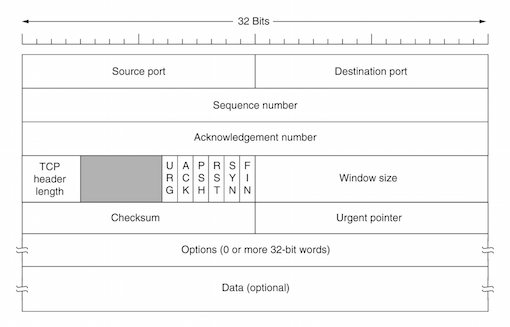
\includegraphics[width=\textwidth]{img/tcp2.png}}
	\caption{Uspořádání TCP packetu}
	\label{fig:tcp-packet}
\end{figure}

%\begin{figure}[H]
%   \centering
%	\makebox[\textwidth]{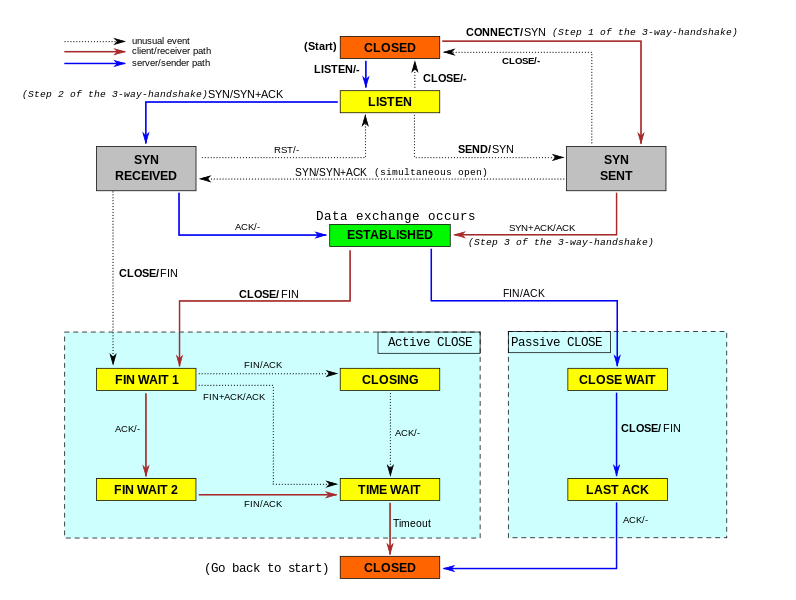
\includegraphics[width=\textwidth]{img/tcp.png}}
%	\caption{TCP stavový diagram}
%	\url{http://commons.wikimedia.org/wiki/File:Tcp_state_diagram_fixed_new.svg}
%	\label{fig:tcp}
%\end{figure}

\section{UDP}
UDP \index{UDP} je oproti TCP protokol typu \uv{fire and forget}, tedy informace se vyšle a v tu chvíli se zdrojové zařízení přestává o tuto informaci starat. Zdrojové zařízení pak neví, jestli informace dorazila na místo určení, nebo nikoliv. To má za následek určitou nespolehlivost přenosu informace, ale o mnohem méně režie potřebné pro přenos. V porovnání s TCP přenáší UDP datagram mnohém méně informace v záhlaví:

\begin{figure}[H]
    \centering
	\makebox[\textwidth]{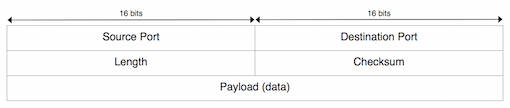
\includegraphics[width=\textwidth]{img/udp.png}}
	\caption{Uspořádání UDP datagramu}
	\label{fig:udp-datagram}
\end{figure}

Pro poslání informace potom stačí vyslat jeden tento datagram s daty a to je vše. Proto skutečnost, že neznáme výsledek přenosu vede k tomu, že musíme být smířeni s faktem, že se některé datagramy při přenosu jednoduše ztratí. Tento problém nastane až u větších sítí, ale při praktickém testování tohoto projektu se ukázalo, že může dojít ke ztrátě datagramů na levnějších komponentách sítě, v tomto případě mohl za ztráty switch. Tento nežádoucí stav může nastat buď vlivem malé paměti daného zařízení, nebo vysokou rychlostí posílání datagramů, což je hlavní příčina. Na levnějších zařízeních pak dochází k přenosu pouze nejrychlejšího náhodného datagramu. Celá síť se pak chová tak, že se datagramy posílají na náhodné prvky za tímto switchem, ale nikdy ne na více než jedno zařízení. Tento efekt byl pozorován na zařízeních ZyXEL ES-105A i TP-LINK TL-WR743ND. U switche D-Link DFE-916DX k tomuto efektu nedošlo.

Tento přenos (vzhledem k charakteru UDP) je tedy vhodný pro přenos velkého množství informací s tím, že nám případné ztráty nevadí. Typickým zástupcem toho typu přenosu jsou například kontinuální čidla, která neustále snímají (například teplotu) a v krátkých časových intervalech posílají informace na server.